\documentclass[xcolor={dvipsnames}]{beamer}
\usepackage{import}
\import{C:/Users/ryanj/Dropbox/code/LatexMacros/}{mymacros2.tex}

\usetheme{metropolis}
\usecolortheme[snowy]{owl}


\title{ Week 8 and 9 Discussion Section Questions}
\subtitle{Questions 7.9, 7.2 and 7.14}
\author{Ryan Martin}


\begin{document}

	\maketitle


	\begin{frame}{Table of Contents}
		\tableofcontents
	\end{frame}

	\section{Question 1}
	
	\begin{frame}[allowframebreaks]{7.9}
	In the STAR experiment (Section 7.5.3), children were randomly assiged within schools into three types of c lasses: small classes with 13-17 students, regular-sized classes with 22-25 students, and regular-sized classes with a full-time teacher aide to assist the teacher. Student scores on acheievement tests were recorded, as was some information about the students, teachers and schools. Data e kindergarten classes is contained in the data file \texttt{star.dat}
	
	\begin{itemize}
		\item[a] Calculate the average of TOTALSCORE for (i) students in regular-sized classrooms with full time teachers, but no aide; (ii) students in regular-sized classrooms with full time teachers and an aide; and (iii) students in small classrooms. What do you observe about test scores in these three types of learning environments?
		
		
		\item[b] Estimate the regression model $$TOTALSCORE_i = \beta_1 + \beta_2 SMALL_i + \beta_3 AIDE_i + e_i$$
		\item[c] Use a t-test to test the hypothesis $H_0: \beta_2 \ge 1$ against the alternative $H_1: \beta_2 < 1$
		
		\item[c] To the regression in (b) add the additional explanatory variable TCHEXPER. Is this variable statistically significant? Does its addition to the model affect the estimates of $\beta_2$ and $\beta_3$?
		
		\item[d] To the regression in (c) add the additional explanatory variables BOY, FREELUNCH and WHITE\_ASIAN. Are any of these variables statistically significant? Does their addition to the model affect the estimates of $\beta_2$ and $\beta_3$?
		
		\item[e] To the regression in (d), add the additional explanatory variables TCHWHITE, TCHMASTERS, SCHURBAN and SCHRURAL. Are any of these variables statistically significant? Does their addition to the model affect the estimates of $\beta_2$ and $\beta_3$?
		
		\item[f] Discuss the importantce of parts (c), (d) and (e) to our estimation of the ``treatment'' effects in part(b).
		
		\item[g] Add to the models in (b) through (e) indicator variables for each school.
		
		$$SCHOOL_{j} = \begin{cases} 1 \text{ if student is in school } j \\ 0 \text{ otherwise} \end{cases}$$ Test the significance of these school ``fixed effects.'' Does the inclusion of these fixed effect indicator variables substantially alter the estimate of $\beta_2$ and $\beta_3$ 
		
		
	\end{itemize}
	
\end{frame}
	
	
	\section{Question 2}
	
	\begin{frame}[allowframebreaks]{7.2}
	In September 1998, a local TV station contacted an econometrician to analyze some data for them. They were going to do a Halloween story on the legend of full mons' affecting behavior in strange ways. They collected data from a local hospital on emergency room cases for the period from January 1, 1998 until mid-August. There were 229 observations (days). During this time, there were eight full moons and seven new moons ( a related myth concerns new moons) and three holidays (NYD, Memorial Day and Easter). If there is a full-moon effect, then hospital administrators will adjust numbers of emergency room doctors and nurses and local police may change the number of officers on duty. (This sounds like a very 90s era question.)
	
	Using the data in the file \texttt{fullmoon.dat} we obtain the regression results in the following table: T is a time trend (T = 1, 2, 3, ..., 229) and the rest are indicator variables. $HOLIDAY = 1$ if the day is a holiday; 0 otherwise. $NEWMOON = 1$ if there is a new moon; 0 otherwise.
	
	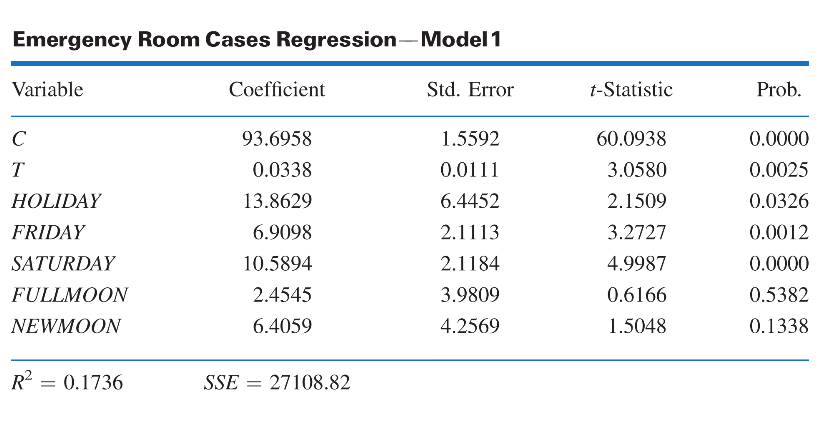
\includegraphics{TableMoonReg.png}
	
	\begin{itemize}
		\item[a] Interpret these regression results. When should emergency rooms expect more calls?
		
		\item[b] The model was reestimated omitting the variables FULLMOON and NEWMOON, as shown below. Comment on any changes you observe.
		
		\item[c] Test the joint significance of FULLMOON and NEWMOON. State the null and alternative hypotheses and indicate the test statistic you use. What do you conclude?
		
	\end{itemize}

	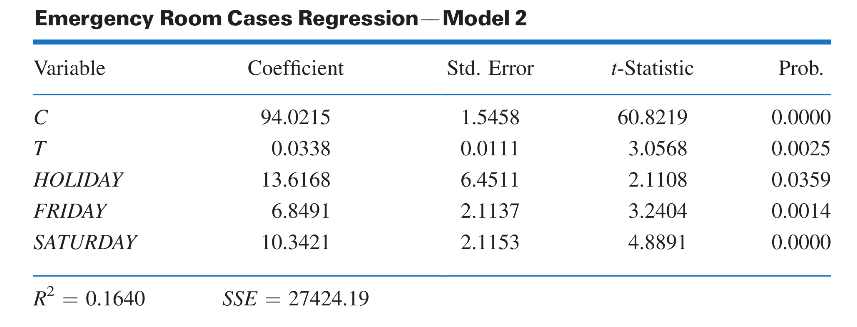
\includegraphics{TableMoonReg2.png}
	
\end{frame}


	\section{Question 3}
\begin{frame}[allowframebreaks]{7.14}
	Professor Ray C. Fair's voting model was introduced in Exercise 2.14. He builds models that explain and predict the U.S. presidential elections. See his website at \url{http://fairmodel.econ.yale.edu/vote2008/index2.htm}. The basic premise of the model is that the incumbent party's share fo the two-party popular vote is affected by a number of factors relating to the economy and variables relating to the politics, such as how long the incumbent party has been in power and whether the president is running for reelection. Fair's data, 33 observations for the election years from 1880 to 2008, are in the file \texttt{fair4.dat}. The dependent variable is VOTE = percentage share of the popular vote won by the incumbent party. The explanatory variables include:
	\begin{itemize}
		\item PARTY: Binary variable that's either 1 or -1. 1 if Democratic incumbent, -1 if Republican.
		\item PERSON: binary (0-1), 1 if incumbent is runing for (re)election.
		\item DURATION: discrete variable. 0 if the incumbent party has been in power for one term, 1 if the incumbent party has been in power for two consecutive terms, 1.25 if the incumbent has been in power for three consecutive terms, 1.50 for four, etc.
		\item WAR. binary (0-1). 1 in 1920, 1944, 1948. 0 otherwise
		\item GROWTH: growth rate of real per capita GDP in the first 3 quarters of the election year (annual rate). 
		\item INFLATION: absolute value of the growth rate of GDP deflator in first 15 quarters of the administration (annual rate) except for 1920, 1944 and 1948 (where values are 0).
		\item GOODNEWS: The number of quarters in the first 15 quarters of the administration in which the growth rate of real per capita GDP is greater than 3.2\% at an annual rate, except for 1920, 1944 and 1948, where the values are 0.
	\end{itemize}
	
	\begin{itemize}
		\item[a] Consider the model $$VOTE = \beta_1 + \beta_2 GROWTH + \beta_3INFLATION + \beta_4 GOODNEWS + \beta_5 PERSON + \beta_6 DURATION + \beta_7 PARTY + \beta_8 WAR + e$$ Discuss the anticipated effects of the dummy variables PERSON and WAR

	\item[b] The binary variable PARTY is somewhat different from the dummy variables we have considered. Write out the regression function E(VOTE) for the two values of PARTY. Discuss the effects of this specification.
	\item[c] Use the data for the period 1916-2004 to estimate the proposed model. Discuss the estimation results. Are the signs as expected? Are the estimates statistically significant? How well does the model fit the data? 
	
	\item[d] Predict the outcome of the 2008 election using the given 2008 data for values of the explanatory variables. Based on the prediction, would you have picked the outcome of the election correctly?
	
	\item[e] Construct a 95\% prediction interval for the outcome of the 2008 election. 
	
	\item[f] Using data values of your choice (you must explain them), predict the outcome of the 2012 election.
\end{itemize}

\end{frame}




\end{document}
